\documentclass[12pt,a4paper]{article}
\usepackage[utf8]{inputenc}
\usepackage[francais]{babel}
\usepackage[colorlinks=true,linkcolor=black,linktoc=all]{hyperref}
\usepackage[linesnumbered, ruled, french,onelanguage]{algorithm2e}
\usepackage{graphicx}
\usepackage[T1]{fontenc}
\usepackage{amsmath}
\usepackage{amssymb}
\usepackage{cases}
\usepackage[left=1.5cm,right=1.5cm,top=1.5cm,bottom=1.5cm]{geometry}
\usepackage{pst-node}
\setlength{\parindent}{0pt}
\newcommand\tab[1][0.65cm]{\hspace*{#1}}
\begin{document}
\begin{titlepage}
	\centering
	
\includegraphics[width=0.5\textwidth]{UPMC.png}\par\vspace{1cm}
	{\scshape\LARGE Université Pierre-et-Marie-Curie \par}
	\vspace{1cm}
	{\scshape\large Master d'informatique \par}
	\vspace{1cm}
	{\scshape\Large 4I019 - Complexité, Algorithmes Randomisés et Approchés\par}
	\vspace{1.5cm}
	{\Large\itshape Fanny Pascual\\Damien Vergnaud\par}
	\vspace{2cm}
	{\huge\bfseries Notes de cours\par}
	\vfill
	Écrit par B.T. Luong\par 
	\vfill
\end{titlepage}
\newpage
\tableofcontents
\newpage
\part{Introduction à la théorie du calcul et à la complexité des problème, Méthodes arborescentes, et Algorithmes d'approximation}
\section{Introduction à la théorie du calcul}
\subsection{Problème, algorithme}
\textbf{Problème de décision :}
\begin{itemize}
	\item \textit{D} : ensemble des instances
	\item $D^+$ : ensemble des instances dont la réponse est "oui"
\end{itemize}
Étant donné I $\in D$, est-ce que I $\in$ $D^+$ ?\\\\
3 types de problèmes:
\begin{itemize}
	\item Problème indécidables : Il n'existe pas d'algorithme les résolvant
	\item Problème facile: Il existe un algorithme efficace les résolvant
	\item Problème difficile : on conjecture qu'$\nexists$ d'algorithme efficace les résolvant\\
\end{itemize}
Problèmes indécidables : 
\begin{itemize}
	\item Problème de l'arrêt
	\item Comparaison 2 algorithmes
\end{itemize}
\subsection{Formalisation}
\subsubsection{Problème et langage}
Une machine code des données avec un alphabet $\Sigma$.\\
Ordinateur $\Sigma$ = \{0, 1\}.\\
\textit{Un mot : }suite infinie de symboles de $\Sigma$.\\
$\tab$Exemple : 01100.\\
\textit{Un langage : }ensemble de mots.\\
$\tab$Exemple : $\Sigma$ = \{0, 1, \#\}\\
$\tab$L = \{w\#w | w est un mot sur \{0, 1\}\}\\
$\tab$010\#010 $\in$ L\\
$\tab$010\#010 $\notin$ L\\
Soit L un langage :\\
$\tab$ \textbf{Instance : }un mot x\\
$\tab$ \textbf{Question : }x $\in$ L?
\subsubsection{Machine de Turing}
\textbf{a Description de haut niveau}
\begin{itemize}
	\item Une mémoire : un ruban infini découpé en cases.
	\item Une tête de lecture/écriture
	\item Des règles de fonctionnement qui indiquent ce que fait la tête de lecture
\end{itemize}
Une MT possède un nombre fini d'état dont:
\begin{itemize}
	\item L'état initial
	\item L'état d'acceptation : q accepter
	\item L'état rejet : q rejet
\end{itemize}
\textbf{Instruction}\\
Si je suis dans un état $E_i$ et que je lis un symbole $\alpha$ alors :
\begin{enumerate}
	\item J'écris un symbole $\beta$
	\item Je me déplace d'une case (soit à gauche ou à droite)
	\item Je passe dans l'état $E_j$
\end{enumerate}
\textbf{Description de haut niveau d'une MT}
\begin{itemize}
	\item Se déplacer de la $1^{ere}$ position du mot à gauche du \# à la $1^{ere}$ position du mot à droite du \# et vérifier que ces mots contiennent le même symbole. Si ce n'est pas les cas $\rightarrow$ Rejeter.
	\item Barrer les symboles dès qu'ils sont vérifiés.
	\item Recommencer avec la position suivante tant que tous les symboles à gauche de \# n'ont pas été barrés.
	\item Quand tous les symboles à gauche du \# ont été barrés, regarder s'il existe des symboles à droites du \#. Si c'est le cas rejeter, sinon accepter.\\
\end{itemize}
\textbf{b Définition formelle d'une MT (bas niveau)\\}
Une MT est un 7-uplet :
\begin{enumerate}
	\item Q : L'ensemble des états.
	\item $\Sigma$ : L'alphabet d'entrée (qui contient pas les symbole \textvisiblespace)
	\item $\Gamma$ : L'alphabet du ruban avec \textvisiblespace $\in$  $\Gamma$, et $\Sigma$ $\in$ $\Gamma$
	\item $\delta$ = Q x $\Gamma$ $\rightarrow$ Q x $\Gamma$ x \{G, D\} : La fonction de transition
	\item $q_0$ $\in$ Q : L'état initial
	\item $q_{accepter}$ $\in$ Q
	\item $q_{rejet}$ $\in$ Q ($q_{accepter}$ $\neq$ $q_{rejet}$)
\end{enumerate}
Exemple :\\
E =\{\#$x_1$\#$x_2$...\#$x_n$ est un mot | $x_i$ $\in$ \{0, 1\} et $x_i$ $\neq$ $x_j$ $\forall$ i $\neq$ j\}\\\\
\textbf{c Langage/Problème décidable\\}
Soit M une MT
\begin{itemize}
	\item M accepte un mot w si l'exécution de M sur w conduit à $q_{accepter}$.
	\item M rejette un mot w si l'exécution de M sur w conduit à $q_{rejet}$.\\
\end{itemize}
\textbf{Langage connu par M }= \{w | M accepte w\}\\
\textbf{Un décideur : }MT qui termine pour tout mot w\\
Un langage est \underline{décidé} par une MT s'il existe une MT que le décide.\\
\textbf{Problème indécidable : } $\nexists$ MT qui le décide.\\\\
\textbf{\large Problème de Hilbert}\\
D = \{p | p est un polynôme ayant une racine entière\}\\
p(\textit{x}) = 3$x^2$ + 2\textit{x} - 1 = 0\\
M : "Évaluer p(\textit{x}) avec \textit{x} prenant successivement les valeurs 0, 1, -1, 2, -2, ...\\
Si p(\textit{x}) = 0 pour une de ces valeurs, alors accepter.\\
Plusieurs variables : Polynôme de Matijasevic.\\\\
\textbf{d Machine de Turing universelle\\}
MT qui simule n'importe quelle autre MT.\\
Reconnaît le langage \{<M,w> | M est une MT qui accepte w\} sur l'entrée (M,w).\\
MTU =
\begin{enumerate}
	\item Simule M sur l'entrée w
	\item Si M entre dans un état d'acceptation, accepter.\\Si M entre dans un état de rejet, rejeter.
\end{enumerate}
\textbf{Machine de Turing non déterministe}\\
À chaque itération, la machine ne peut avoir plusieurs actions possibles.\\
\tab $\delta$ = Q x $\Gamma$ $\longmapsto$ P (Q x $\Gamma$ x \{G, D\})\\
Une MTND accepte le mot w $\Leftrightarrow$ Il existe une branche que mène à l'état d'acceptation.\\\\
\textbf{f La thèse de Church Turing (1930 - 1936)}\\
Notion intuitive d'algorithme = MT.\\
Un problème peut être résolu par un algorithme ssi il peut être décidé par une MT.
\section{Complexité de problèmes}
\subsection{Complexité temporelle définie par les machines de Turing}
Soit M une MTD qui est un décideur.\\
La complexité temporelle de M est une fonction f : $\mathbb{N}$ $\longmapsto$ $\mathbb{N}$ où f(n) est le nombre maximum d'étapes que n utilise pour une entrée de talle n.
\subsection{Complexité d'un problème définie par les machines de Turing}
Soit f : $\mathbb{N}$ $\longmapsto$ $\mathbb{R^+}$ une fonction.\\
La classe de complexité TIME(f(n)) = l'ensemble de tous les langages qui sont décidables par une \textit{MTD} qui s'exécute en temps f(n).
\subsection{La classe P}
P = $\bigcup\limits_{k \in \mathbb{N}}$ TIME($n^k$)\\
Ensemble de tous les langages décidables en temps polynomial par une MTD.
\subsection{Temps d'exécutions  d'une machine de Turing non déterministe}
Soit M une MTND qui est un décideur.\\
Le temps d'exécution de M est une fonction f : $\mathbb{N}$ $\longmapsto$ $\mathbb{N}$ où f(n) = nombre maximum d'étapes que M utilise pour n'importe quelle entrée de taille n.\\
Soit f : $\mathbb{N}$ $\longmapsto$ $\mathbb{R^+}$. La classe de complexité NTIME(f(n)) = ensemble de tous les langages décidables par une MTND qui s'exécute en f(n).
\subsection{La classe NP}
NP (non déterministe polynomial) = $\bigcup\limits_{k \in \mathbb{N}}$ NTIME($n^k$)\\
Ensemble des langages décidés en temps polynomiale par une MTND.\\\\
\textit{Proposition :}\\
Un langage L sur un alphabet $\Sigma$ est dans NP si et seulement s'il existe un polynôme p et une MTND M telle que tout mot x de taille n : x $\in$ L $\Leftrightarrow$ $\exists$y (certificat "indice") $\in$ $\Sigma^{p(n)}$, M accepte l'entrée (x,y).
\subsection{Exemple de problème dans NP}
\textbf{\Large CHAÎNE HAMILTONIENNE : CH}\\
\begin{itemize}
	\item \textbf{Entrée :} G.
	\item \textbf{Question :} G possède-t-il une chaîne hamiltonienne ie une chaîne qui passe une fois et une seule fois par chaque sommet de G ?
	\item \textbf{Certificat :} Chaîne hamiltonienne.\\
\end{itemize}
\textbf{\Large CLIQUE}\\
\begin{itemize}
	\item \textbf{Entrée :} Un graphe non orienté G et un entier k.
	\item \textbf{Question :} G possède-t-il \underline{une clique de taille k}? (un ensemble de k sommets 2 à 2 adjacents)
	\item \textbf{Certificat :} Une clique de taille k.\\
\end{itemize}
\textbf{\Large PARTITION}\\
\begin{itemize}
	\item \textbf{Entrée :} S ensemble de n entiers positifs.
	\item \textbf{Question :} Peut-on partitionner S en 2 sous-ensembles $S_1$ et $S_2$ tels que la somme des entiers dans $S_1$ = la somme des entiers dans $S_2$?
	\item \textbf{Certificat :} $S_1$ et $S_2$.\\
\end{itemize}
\textbf{\Large SATISFIABILITÉ (SAT)}\\
\begin{itemize}
	\item \textbf{Entrée :} Une formule booléenne $\phi$.
	\item \textbf{Question :} $\phi$ est-elle satisfiable?
	\item \textbf{Certificat :} Valeurs de vérité (V ou F) aux variables.\\
\end{itemize}
\subsection{P $\lor$ NP}
P $\leftarrow$ problèmes dont on peut rapidement trouver leur solution.\\
NP $\leftarrow$ problèmes dont on peut rapidement vérifier qu'une solution est bien une solution.\\
P $\subset$ NP\\
\textit{Question ouverte : } P $\neq$ NP?
\subsection{Problème NP-complet}
Un problème NP-complet si sa complexité est liée à celle de la classe NP.\\
Un algorithme polynomial résolvant un problème NP-complet permet de résoudre en temps polynomial tout problème de NP.\\\\
\textit{\underline{Théorème} :} SAT $\in$ P $\Leftrightarrow$ P = NP
\subsection{Réduction polynomiale}
Le problème A peut être réduit en temps polynomial au problème B ce qui s'écrit A $\leq_p$ B s'il existe une fonction f exécutable en temps polynomial telle que pour toute instance w de A :\\
\tab La réponse au problème A sur l'instance w est OUI.\\
$\Leftrightarrow$ La réponse au problème B sur l'instance f(w) est OUI.\\
f est une réduction polynomiale de A vers B.\\\\
\textit{\underline{Théorème} :} Si  A $\leq_p$ B et B $\in$ P alors A $\in$ P.\\\\
\underline{Définition :} Soit A un problème de décision.\\
\tab A est NP-complet si :
\begin{enumerate}
	
	\item A $\in$ NP
	\item Chaque problème B de NP peut être réduit en temps polynomial à A
\end{enumerate}
\subsection{Comment montrer qu'un problème est NP-complet}
\textit{\underline{Théorème} :} Si B est NP-complet et B $\leq_p$ A avec A $\in$ NP, alors A est NP-complet.\\
Pour montrer qu'un problème est NP-complet :
\begin{enumerate}
	\item On montre que A $\in$ NP (certificat)
	\item On montre qu'il existe un problème NP-complet B tel que B $\leq_p$ A
\end{enumerate}
\underline{Résumé :}
\begin{enumerate}
	\item Énoncer clairement le problème A dont on veut montrer qu'il est NP-complet.
	\item On montre que A $\in$ NP (certificat).
	\item Énoncer clairement un problème B dont on sait qu'il est NP-complet.
	\item On décrit une réduction polynomiale f qui transforme B en A.
	\item On prouve que f transforme B en A : $\forall$ entrée w de B, on obtient une entrée f(w) de A tel que : la solution au problème B sur l'instance w est OUI $\Leftrightarrow$ la solution au problème A sur l'instance f(w) est OUI.
\end{enumerate}
Exemple : On montre que CLIQUE est NP-complet
\begin{enumerate}
	\item Problème CLIQUE :\\
	\textbf{Entrée :} Un graphe C et un entier k\\
	\textbf{Question :} Est-ce qu'il existe une clique de taille k dans G?
	\item CLIQUE $\in$ NP\\
	\textbf{Certificat : clique de taille k}
	\item Problème 3-SAT :\\
	Une formule booléenne est en forme normale conjonctive (FNC) si elle constitue d'un ensemble de clauses (litéraux reliés par des $\lor$) reliées par des $\land$.\\
	Exemple : ($x_1$ $\lor$ $x_2$) $\land$ ($\overline{x_2}$ $\lor$ $x_3$ $\lor$ $\overline{x_4}$)\\
	Une formule booléenne 3FNC est une formule en FNC telle que chaque clause a 3 littéraux.\\
	Exemple : ($x_1$ $\lor$ $x_2$ $\lor$ $\overline{x_3}$) $\land$ ($x_1$ $\lor$ $x_4$ $\lor$ $\overline{x_2}$)\\
	Problème 3-SAT :\\
	\textbf{Entrée :} Une formule booléenne 3FNC $\phi$\\
	\textbf{Question :} $\phi$ est-elle satisfiable?
	\item On réduit 3-SAT à CLIQUE :\\
	Étant une instance de 3-SAT à m clauses, on construit l'instance de CLIQUE suivant :
	\begin{itemize}
		\item k = m
		\item les sommets de G sont organisés en triples $t_1$, ..., $t_m$
	\end{itemize}
	Chaque triplet correspond à une clause de $\phi$ :\\
	\begin{center}
		$\phi$ = ($x_1$ $\lor$ $x_1$ $\lor$ $x_2$) $\land$ ($\overline{x_1}$ $\lor$ $\overline{x_2}$ $\lor$ $\overline{x_2}$) $\land$ ($\overline{x_1}$ $\lor$ $x_2$ $\lor$ $x_2$)
	\end{center}
	\begin{center}
		\begin{psmatrix}[mnode=circle]
			&$\overline{x_1}$   &$\overline{x_2}$   &$\overline{x_2}$\\
			$x_1$&  &  &  &$\overline{x_1}$\\
			$x_1$&  &  &  &$x_2$\\
			$x_2$&  &  &  &$x_2$
		\end{psmatrix}
		\psset{arrows=-,shortput=nab}
		\ncline{2,1}{1,3}
		\ncline{2,1}{1,4}
		\ncline{2,1}{3,5}
		\ncline{2,1}{4,5}
		\ncline{3,1}{1,3}
		\ncline{3,1}{1,4}
		\ncline{3,1}{3,5}
		\ncline{3,1}{4,5}
		\ncLine[linecolor=red]{4,1}{1,2}
		\ncLine{4,1}{2,5}
		\ncLine[linecolor=red]{4,1}{3,5}
		\ncLine{4,1}{4,5}
		\ncLine{1,2}{2,5}
		\ncLine[linecolor=red]{1,2}{3,5}
		\ncLine{1,2}{4,5}
		\ncLine{1,3}{2,5}
		\ncLine{1,4}{2,5}
	\end{center}
	Les arêtes de G lient tous les sommets sauf ceux qui sont dans un des 2 cas suivant :
	\begin{itemize}
		\item Il n'y a pas d'arête entre 2 sommets d'un même triplet.
		\item Il n'y a pas d'arête entre 2 sommets étiquetés par des littéraux opposés. 
	\end{itemize}
	\item Propriété : Il existe dans G($\phi$) une clique de taille k $\Leftrightarrow$ $\phi$ est satisfiable.\\
	($\Leftarrow$) Supposons que $\phi$ est satisfiable. Donc on a au moins 1 littéral VRAI dans chaque clause. Dans chaque triplet de G on sélectionne un littéral qui a la valeur VRAI dans $\phi$. Les sommets sélectionnés forment une clique de taille k :
	\begin{itemize}
		\item k sommets sélectionnés
		\item chaque paire de sommets est reliée par une arête (pas de 2 sommets est d'un triplet, pas de 2 sommets correspondant à des littéraux opposés)
	\end{itemize}
	($\Rightarrow$) Supposons qu'il existe une clique de taille k dans G($\phi$). Montrons que $\phi$ est satisfiable.
	\begin{itemize}
		\item On n'a pas 2 sommets dans un même triplet.
		\item On associe la valeur VRAI à chaque littéral associé à un sommet de la clique.
	\end{itemize}
	$\phi$ est satisfiable car :
	\begin{itemize}
		\item On n'a pas affecté la valeur VRAI à des littéraux opposés.
		\item On a au moins un littéral VRAI par clause.
	\end{itemize}
\end{enumerate}
\section{Algorithmes approchés à garantie de performance}
\textbf{Problème d'optimisation}
\begin{itemize}
	\item \textbf{Entrée :} I
	\item \textbf{Fonction objective f :} $A_I$ $\longmapsto$ $\mathbb{R}$
\end{itemize}
$\star$ Trouver un élément $\overline{x}$ de $A_i$ tel que f($\overline{x}$) $\leq$ f(x) $\forall$ x $\in$ $A_I$. (problème de minimisation)\\
$\star$ Trouver un élément $\overline{x}$ de $A_i$ tel que f($\overline{x}$) $\geq$ f(x) $\forall$ x $\in$ $A_I$. (problème de maximisation)\\\\
\textbf{Problème de décision associé}
\begin{itemize}
	\item \textbf{Entrée :} I, borne B
	\item \textbf{Fonction objective f :} $A_I$ $\longmapsto$ $\mathbb{R}$
\end{itemize}
$\star$ Est-ce qu'il existe un élément x $\in$ $A_I$ tel que f(x) $\leq$ B ? (problème de minimisation)\\
$\star$ Est-ce qu'il existe un élément x $\in$ $A_I$ tel que f(x) $\geq$ B ? (problème de maximisation)\\\\
\textbf{Un problème d'optimisation est NP-difficile si le problème de décision associé est NP-complet.}\\\\
Un algorithme est $\alpha$-approché s'il retourne pour chaque instance du problème une solution dont le coût est :
\begin{itemize}
	\item au plus $\alpha$ OPT pour un problème de minimisation
	\item au moins $\alpha$ OPT pour un problème de maximisation
\end{itemize}
où OPT la valeur d'une solution optimale et $\alpha$ le rapport d'approximation.\\\\
Exemple: MAX SAT\\
\tab Entrée : Une forme FNC $\phi$.\\
\tab But : Maximiser le problème de clauses satisfiables dans $\phi$.\\
\tab Exemple : ($x_1$ $\lor$ $\overline{x_2}$ $\lor$ $\overline{x_3}$) $\land$ ($x_2$ $\lor$ $x_1$) $\land$ $\overline{x_2}$ $\land$ ($\overline{x_2}$ $\lor$ $\overline{x_1}$)\\
\tab Algorithme :
\begin{enumerate}
	\item Affecter toutes les variables à VRAI $\Rightarrow$ $m_1$ clauses satisfiables.
	\item  Affecter toutes les variables à FAUX $\Rightarrow$ $m_2$ clauses satisfiables.
\end{enumerate}
\tab Retourner l'affectation qui satisfait le plus de clauses : \#Clauses satisfaites = $\max$ \{$m_1$, $m_2$\}
\begin{center}
	$m_1$ + $m_2$ $\geq$ m $\Rightarrow$ $\max$ \{$m_1$, $m_2$\} $\geq$ $\dfrac{m}{2}$ $\geq$ $\dfrac{OPT}{2}$
\end{center}
\tab Or OPT $\leq$ m\\
\tab Cet algorithme est $\dfrac{1}{2}$-approché.\\\\
\textbf{\underline{3 catégories de problème d'optimisation}}
\begin{enumerate}
	\item Les problèmes non-approximables\\
	$\nexists$ d'algorithme polynomial $\alpha$-approché, $\forall$$\alpha$ constante, si P $\neq$ NP.
	\item Les problèmes approximables\\
	Il existe une constante $\alpha$ telle qu'il existe algorithme polynomial $\alpha$-approché.
	\item Les problèmes totalement approximables\\
	Un schéma d'approximation est pour un problème P est un algorithme qui prend en entrée :
	\begin{itemize}
		\item une instance I de P
		\item un nombre $\epsilon$ > 0 (précision souhaitée)
	\end{itemize}
	et qui retourne une solution SA dont le coût est tel que :
	\begin{itemize}
		\item coût ($S_A$) $\geq$ (1 - $\epsilon$) OPT si P est un problème de maximisation.
		\item coût ($S_A$) $\leq$ (1 + $\epsilon$) OPT si P est un problème de minimisation.\\
	\end{itemize}
\end{enumerate}
Exemple :\\
\textbf{\Large Problème VOYAGEUR DE COMMERCE (VC)}\\
\tab \textbf{Entrée :} G un graphe complet G = {S, A} dont les arêtes sont valuées par un coût $\geq$ 0.\\
\tab \textbf{Question :} Trouver un cycle hamiltonien de coût minimum.\\
\textit{\underline{Théorème} :} $\forall$ constante $\alpha$, $\nexists$ d'algorithme $\alpha$-approché polynomial pour le problème VC sauf si P = NP.\\
\textbf{Preuve :}\\
\textbf{Idée :} Réduction CYCLE HAMILTONIENNE $\Rightarrow$ VC\\
Soit A un algorithme polynomial $\alpha$-approché pour VC.\\
On suppose P $\neq$ NP.\\
On transforme G : entrée VC $\Rightarrow$ G' : entrée CH, telle que :
\begin{itemize}
	\item Si G' admet un cycle hamiltonien alors le coût optimal du VC dans G est n.
	\item Sinon le coût optimal du VC dans G > $\alpha$n.
\end{itemize}
\textbf{Réduction :}\\
G :
\begin{itemize}
	\item même que G'
	\item arête a un coût 1 ssi \{u, v\} appartient à G'
	\item sinon \{u, v\} a un coût $\alpha$n
\end{itemize}
Supposons qu'il existe un algorithme polynomial $\alpha$-approché pour le problème du VC.\\
\textbf{Réduction :}\\
CYCLE HAMILTONIEN (NP-'complet)\\
\tab \textbf{Entrée :} Graphe G ) (S, A)\\
VOYAGEUR DE COMMERCE\\
\tab \textbf{Entrée} C' = (S', A) aec S' = S\\
Pondération $\forall$\{u, v\} $\in$ A'
\begin{itemize}
	\item Si \{u, v\} $\in$ A alors coût(\{u, v\}) = 1
	\item Sinon coût(\{u, v\}) = $\alpha$n
\end{itemize}
$\mathcal{A}$ permet de détecter un cycle hamiltonien dans G.
\begin{itemize}
	\item Si G contient un cycle hamiltonien $\Rightarrow$ OPT = n\\
	\begin{center}
		\begin{tabular} {c c c c}
			G: &
			\begin{psmatrix}[mnode=circle]
				1& 2\\
				4& 3
			\end{psmatrix}
			\psset{arrows=-,shortput=nab}
			\ncline{1,1}{1,2}
			\ncLine{1,1}{2,1}
			\ncline{1,2}{2,2}
			\ncline{2,1}{2,2}
			\ncline{1,2}{2,1}&
			$\Rightarrow$ G': &
			\begin{psmatrix}[mnode=circle]
				1& 2\\
				4& 3
			\end{psmatrix}
			\psset{arrows=-,shortput=nab}
			\ncline{1,1}{1,2}^{1}
			\ncLine{1,1}{2,1}^{1}
			\ncline{1,2}{2,2}^{1}
			\ncline{2,1}{2,2}^{1}
			\ncline{1,2}{2,1}^{1}
			\ncline[linecolor=red]{1,1}{2,2}^{\color{red}$\alpha$n}
		\end{tabular}
	\end{center}
	$\newline$
	$\Rightarrow$ $\mathcal{A}$ retourne une solution de coût $\leq$ $\alpha$n.
	\item Si G ne contient pas de cycle hamiltonien, la solution optimale du VC utilise au moins 1 arête de coût $\alpha$n $\Rightarrow$ OPT > $\alpha$n
	\begin{center}
		\begin{tabular} {c c c c}
			G: &
			\begin{psmatrix}[mnode=circle]
				1& 2\\
				4& 3
			\end{psmatrix}
			\psset{arrows=-,shortput=nab}
			\ncline{1,1}{1,2}
			\ncLine{1,1}{2,1}
			\ncline{1,2}{2,2}
			\ncline{1,2}{2,1}&
			$\Rightarrow$ G': &
			\begin{psmatrix}[mnode=circle]
				1& 2\\
				4& 3
			\end{psmatrix}
			\psset{arrows=-,shortput=nab}
			\ncline{1,1}{1,2}^{1}
			\ncLine{1,1}{2,1}^{1}
			\ncline{1,2}{2,2}^{1}
			\ncline[linecolor=red]{2,1}{2,2}^{\color{red}$\alpha$n}
			\ncline{1,2}{2,1}^{1}
			\ncline[linecolor=red]{1,1}{2,2}^{\color{red}$\alpha$n}
		\end{tabular}
	\end{center}
	$\newline$
	$\Rightarrow$ $\mathcal{A}$ répond en temps polynomial de problème du cycle hamiltonien.\\
\end{itemize}
Donc P = NP $\Rightarrow$ Contradiction.
\section{Méthodes arborescents exactes et approchées}
\textbf{\large Voyageur de commerce dans un graphe métrique}\\
Algorithme 2-approché :\\
Soit G = (S, A)\\
Inégalité triangulaire : $\forall$ triplet (a, b, c) $\in$ $S^3$
\begin{center}
	coût (\{a, b\}) $\leq$ coût (\{b, c\}) + coût (\{c, a\})
\end{center}
Algorithme
\begin{enumerate}
	\item Calculer un arbre courant de coût minimum, T de G.\\{\color{blue} coût(T) $\leq$ OPT}
	\item Dupliquer chaque arête de T pour obtenir un graphe eulérien T'.\\{\color{blue} coût(T') = 2coût(T) $\leq$ 2OPT}
	\item Calculer un cycle eulérien de T'.\\{\color{blue} coût(C) = coût(T') $\leq$ 2OPT}
	\item Retourner $\mathcal{C}$ le cycle qui passe par tous les sommets de G.\\{\color{blue} coût($\mathcal{C}$) $\leq$ coût(C) (inégalité triangulaire)}\\
	$\Rightarrow$ Donc {\color{red} coût($\mathcal{C}$) $\leq$ 2OPT}
\end{enumerate}
L'algorithme est 2-approché.\\
\begin{center}
	\begin{psmatrix}[mnode=circle]
		& B & & D\\
		A & & C\\
		& & E\\
		& G & & F
	\end{psmatrix}
	\psset{arrows=-,shortput=nab}
	\ncline{2,1}{1,2}
	\ncLine{1,2}{2,3}
	\ncLine{2,3}{1,4}
	\ncLine{2,3}{3,3}
	\ncLine{3,3}{4,2}
	\ncLine{3,3}{4,4}
	\ncarc[arcangle=-30, linecolor=blue]{2,1}{1,2}
	\ncarc[arcangle=-30, linecolor=blue]{1,2}{2,3}
	\ncarc[arcangle=-30, linecolor=blue]{2,3}{1,4}
	\ncarc[arcangle=30, linecolor=blue]{2,3}{3,3}
	\ncarc[arcangle=-30, linecolor=blue]{3,3}{4,2}
	\ncarc[arcangle=-30, linecolor=blue]{3,3}{4,4}
	\ncarc[arcangle=30, linecolor=red]{2,1}{1,2}
	\ncarc[arcangle=30, linecolor=red]{1,2}{2,3}
	\ncarc[arcangle=30, linecolor=red]{2,3}{1,4}
	\ncarc[arcangle=30, linecolor=red]{1,4}{3,3}
	\ncarc[arcangle=30, linecolor=red]{3,3}{4,4}
	\ncarc[arcangle=30, linecolor=red]{4,4}{4,2}
	\ncarc[arcangle=30, linecolor=red]{4,2}{2,1}
	\newline \newline \newline
	--- T\\
	{\color{blue} --- T'}\\
	{\color{red} --- $\mathcal{C}$}\\
	C = (A, B, C, D, C, E, F, E, G, E, C, B, A)\\
	$\mathcal{C}$ = (A, B, C, D, E, F, G, A)
\end{center}
Soit OPT la valeur d'une solution optimale du VC.\\
On a coût(T) $\leq$ OPT.\\
Tour optimal de coût OPT.\\
On lui retire une arête.
On obtient O' de coût O' $\leq$ OPT et coût O'$\geq$ coût(T).\\\\
\textbf{\large Problème du Sac à dos}\\
Schéma d'approximation algorithme (1 - $\epsilon$)-approché.\\
Polynomial en la taille d'entrée et $\dfrac{1}{\epsilon}$.\\
Algorithme pseudo-polynomial dont le temps d'exécution est, pour tout instance I, bornée par un polynôme de taille de I dans laquelle les nombres sont codés en unaire.\\
Soit OPT la valeur des objets dans une solution optimale, $V_{max}$ la valeur maximale d'un objet de S.\\
On a n$V_{max}$ $\geq$ OPT.\\
Soit i $\in$ \{1, ..., n\} et v $\in$ \{0, 1, ..., n$V_{max}$\}.\\
Soit $S_{iv}$ un sous-ensemble de \{$a_1$, ..., $a_i$\} de valeur v et de poids minimum.\\
P(i, v) : poids cumulé des objets de $S_{iv}$ (P(i, v) = +$\infty$ si $S_{iv}$ n'existe pas).\\
\begin{tabular} {lll}
	On a : & P(1, 0) = & 0\\
		   & P(1, v) = & poids($a_1$) si v = val($a_1$)\\
		   & $\forall$ v $\neq$ 0 & $\infty$ sinon
\end{tabular}
Exemple : Sac à dos
\begin{itemize}
	\item Capacité B = 6
	\item Objets B = \{$a_1$, ..., $a_6$\}
\end{itemize}
\begin{center}
	\begin{tabular} {l|llll}
		B	& $a_1$ & $a_2$ & $a_3$ & $a_4$\\\hline
		Poids& 2 & 7 & 1 & 2\\\hline
		Val & 1 & 4 & 2 & 2
	\end{tabular}
	\begin{tabular} {l|llllllllllllllll}
		& 0 & 1 & 2 & 3 & 4 & 5 & 6 & 7 & 8 & 9 & 10 & 11 & 12 & 13 & 14 & 15\\\hline
		\{$a_1$\} & 0 & 2 & $\infty$ & $\infty$ & $\infty$ & $\infty$ & $\infty$ & $\infty$ & $\infty$ & $\infty$ & $\infty$ & $\infty$ & $\infty$ & $\infty$ & $\infty$ & $\infty$\\\hline
		\{$a_1$, $a_2$\} & 0 & 2 & $\infty$ & $\infty$ & 7 & 9 & $\infty$ & $\infty$ & $\infty$ & $\infty$ & $\infty$ & $\infty$ & $\infty$ & $\infty$ & $\infty$ & $\infty$\\\hline
		\{$a_1$, $a_2$, $a_3$\} & 0 & 2 & 1 & 3 & 7 & 9 & 8 & 10 & $\infty$ & $\infty$ & $\infty$ & $\infty$ & $\infty$ & $\infty$ & $\infty$ & $\infty$ \\\hline
		\{$a_1$, $a_2$, $a_3$, $a_4$\} & 0 & 2 & 1 & 3 & 3 & {\color{red} 5} & 8 & 10 & 10 & 12 & $\infty$ & $\infty$ & $\infty$ & $\infty$ & $\infty$ & $\infty$\\
		& & & & & & {\color{red} OPT}
	\end{tabular}
\end{center}
\begin{tabular} {ll}
	P(i + 1, v) = & P(i, v) si val($a_{i + 1}$) > v\\
	& min \{P(i, v), poids($a_{i + 1}$) + P(i, v) - val($a_{i + 1}$)\} sinon
\end{tabular}
\newline
OPT = max \{v= P(i, v) $\leq$ B\}\\
{\color{red} Complexité : $\Theta$ (n * (n$V_{max}$ + 1)) = $\Theta$ ($n^2$$V_{max}$)}\\
\textbf{Un schéma d'approximation totalement polynomial}\\
\begin{enumerate}
	\item Étant donné $\epsilon$ > 0, poser K = $\dfrac{\epsilon V_{max}}{n}$ $\Rightarrow$ $\dfrac{V_{max}}{k}$ = $\dfrac{n}{\epsilon}$
	\item Pour chaque objet a, poser valeur ($a_i$) = $\lfloor \dfrac{valeur(a_i)}{K} \rfloor$
	\item Lancer l'algorithme de programmation dynamique avec ces nouvelles valeurs arrondies et trouver un ensemble S' de valeur maximum.
	\item Retourner S'.
\end{enumerate}
\textbf{\underline{Théorème} :} Cet algorithme est un schéma d'approximation.\\
{\color{red} Complexité : O (n * n$V_{max}$') = O (n * n$\lfloor \dfrac{V_{max}}{K} \rfloor$) = O (n * n$\lfloor \dfrac{n}{\epsilon} \rfloor$) = O ($\dfrac{n^3}{\epsilon}$)}\\\\
On montre maintenant que valeur(S') $\geq$ (1 - $\epsilon$) OPT.\\
Notons val($a_i$) la vraie valeur et val'($a_i$) la valeur arrondie.
\begin{itemize}
	\item $V_{max}$ $\leq$ OPT
	\item Soit X un sous-ensemble d'objets
	\item Soit $a_i$ $\in$ X : val($a_i$) = K val'($a_i$) + $x_i$ avec 0 $\leq$ $x_i$ $\leq$ K
\end{itemize}
Définition :\\
\tab val(X) = $\displaystyle \sum_{a_i \in X}$ val($a_i$)\\
\tab val'(X) = $\displaystyle \sum_{a_i \in X}$ val'($a_i$)\\
On a :
\begin{center}
	{\color{blue} val(X) = Kval'(X) + $\sum$ $x_i$ avec 0 $\leq$ $\sum$ $x_i$ $\leq$ nK}
\end{center}
Ceci est vrai pour X = S'.\\
Donc :\\
{\color{blue}
	\begin{equation}
		\begin{split}
			val(S') \geq Kval'(S')
		\end{split}
	\end{equation}}
Ceci est vrai pour X = O, où O est sous-ensemble d'objets d'une solution optimale.
\begin{center}
	val(O) = Kval'(O) + $\sum$$x_i$
\end{center}
{\color{blue}
	\begin{equation}
		\begin{split}
			Kval'(O) \geq & \underbrace{val(O)} - nK\\
						  & = OPT
		\end{split}
	\end{equation}}
De plus, on a :
{\color{blue}
	\begin{equation}
		\begin{split}
			val'(S') \geq val'(O)
		\end{split}
	\end{equation}}
car S' est la solution optimale du problème avec les valeurs arrondies.\\
On a donc :
{\color{red}
	\begin{align*}
		val(S') &\geq_1 Kval'(S')\\
				&\geq_3 Kval'(O)\\
				&\geq_2 val(O) - nk = OPT - \epsilon V_{max}\\
				&\geq (1 - \epsilon) OPT
	\end{align*}}
\newpage
\part{Algorithmes probabilistes, classes de complexité probabilistes}
\section{Algorithme probabiliste}
\subsection{Introduction}
Aiguille de Buffon (1773) - Proposition d'une expérience aléatoire :\\
Si on prend ces "aiguilles" de longueur d, si les lancers d'aiguilles sont "indépendants" et si le nombre de lancers est suffisamment grand, le quotient du nombre d'aiguilles touchant une ligne par le nombre d'aiguilles total tend vers $\frac{2}{\pi}$.\\
\url{http://www.ventrella.com/buffon/}\\
Méthode de Monté Carlo (1947)\\
Métropolis et Ulam : une autre approche pour calculer $\pi$.\\
On peut tirer au hasard des points (x,y) dans le carré 0 $\leq$ x $\leq$ 1, 0 $\leq$ y $\leq$ 1 et compter ceux qui sont à distances inférieure à 1 de l'origine (i.e. $x^2$ + $y^2$ $\leq$ 1).\\
Le quotient du nombre de points à l'intérieur du quart de cercle par le nombre de points total tend vers $\frac{\pi}{4}$.\\
Utilisation de l'aléatoire en algorithmique :
\begin{itemize}
	\item Éviter les pires des cas d'exécution d'un algorithme\\
	$\rightarrow$ Tri rapide
	\item Échantillonner\\
	$\rightarrow$ Choix du pivot dans le tri rapide
	\item Hachage\\
	$\rightarrow$ Rabin-Karp\\
	$\rightarrow$ Filtre de Bloom
	\item Structure de données aléatoire (tarbres (treaps), liste de décomposition (split lists))
	\item Casser la symétrie
	\item etc.
\end{itemize}
\subsection{Un premier exemple : recherche dans un tableau binaire}
\textbf{Problème (Recherche binaire)}\\
\textbf{Entrée :} T un tableau binaire de longueur paire n qui contient $\frac{n}{2}$ éléments 0 et $\frac{n}{2}$ éléments 1.\\
\textbf{Sortie :} i $\in$ \{1, .., n\} tel que T[i] contient un 1.
\subsubsection{Algorithme déterministe}
\textbf{Proposition :} Il existe un algorithme déterministe qui résout le problème de recherche binaire en regardant $\frac{n}{2}$ cases dans le tableau.\\
\underline{Démonstration :}\\
\begin{algorithm}[H]
	\For{i := 1 $\to$ $\frac{n}{2}$}{
		\If{T[i] == 1}{\Return i}}
	\Return $\frac{n}{2}$ + 1
\end{algorithm}
\textbf{Proposition :} Il n'existe pas d'algorithme déterministe qui résout le problème de recherche binaire en regardant moins de $\frac{n}{2}$ - 1 cases dans le tableau.\\
\underline{Démonstration :}\\
Pour démontrer cette borne inférieure (de complexité), on utilise \underline{la méthode de l'adversaire}.\\
Pour tout algorithme A qui tente de résoudre le problème de recherche binaire en $\frac{n}{2}$ - 1 accès au tableau, on construit un algorithme B qui construit une entrée pour A sur la quelle A va échouer.\\
A accède à certaines cases du tableau $i_1$, $i_2$, .., $i_{\frac{n}{2}-1}$ $\in$ \{1, .., n\} (où la requête $i_j$ peut prendre du contenu des cases T[$i_1$], T[$i_2$], ..., T[$i_{j-1}$]). L'algorithme B construit le tableau de sorte que T[$i_j$] = 0 pour j $\in$ \{1, .., $\frac{n}{2}$ - 1\}.\\
L'algorithme A retourne un indice $i^*$ comme réponse et B peut fixer T[$i^*$] = 0 et l'algorithme A échoue sur l'entrée ainsi construite (qui vérifie les contraintes du problème).
\subsubsection{Algorithmes probabilistes}
Nous considérons les 2 algorithmes suivants :\\
\begin{algorithm}[H]
	\caption{$A_1$}
	i $\xleftarrow{R}$ \{1, .., n\}\\
	\tcc{on tire une valeur uniformément aléatoire et dans \{1, .., n\} et on assigne le résultat à i}
	\While{T[i] == 0}{i $\xleftarrow{R}$ \{1, .., n\}}
	\Return i
\end{algorithm}
\begin{algorithm}[H]
	\caption{$A_2$}
	c $\gets$ 0\\
	i $\xleftarrow{R}$ \{1, .., n\}\\
	\While{T[i] == 0 et c < k}{i $\xleftarrow{R}$ \{1, .., n\}\\c $\gets$ c + 1}
	\Return i
\end{algorithm}
\textbf{Remarques :}\\
L'algorithme $A_1$ retourne toujours un indice i tel que T[i] = 1 mais nous n'avons aucune garantie qu'il termine.\\
Notons $X_i$ la variable aléatoire définie par :
\begin{itemize}
	\item $X_i$ = 1 si la boucle est exécutée au moins i fois
	\item $X_i$ = 0 sinon
\end{itemize}
Le temps d'exécution de l'algorithme en moyenne (pour toute entrée) est :
\begin{center}
	$\sum\limits_{i = 0}^{\infty}$ Pr($X_i$ = 1) = $\sum\limits_{i = 0}^{\infty}$ $\dfrac{1}{2^i}$ = 2
\end{center}
Un tel algorithme (qui retourne toujours une solution et dont le temps d'exécution en moyenne est borné) est dit de type \underline{Las Vegas}.\\
L'algorithme $A_2$ termine toujours en exécutant la boucle au plus k fois (indépendamment de ces choix aléatoires). Par contre, il retourne un indice i tel que T[i] = 0 (i.e. il se trompe) avec une probabilité $\frac{1}{2^{k+1}}$. Un tel algorithme est de type \underline{Monté Carlo}.\\
Il existe d'autres types d'algorithmes probabilistes (notamment \underline{Atlantic City} ou \underline{Bellagio}).
\subsection{Algorithme de sélection}
Nous considérons les 2 problèmes suivants :\\
\textbf{Problème :} Sélection\\
\textbf{Entrée :}
\begin{itemize}
	\item T un tableau d'entiers de longueur n ne contenant que des entiers 2 à 2 distincts.
	\item k $\in$ {1, .., n}
\end{itemize}
\textbf{Sortie :} L'élément T[i] de T qui est de rang k (i.e. tel que T contienne exactement k - 1 éléments inférieur à T[i]).\\
\textbf{Problème :} Sélection $\epsilon$ - approché\\
\textbf{Entrée :} identique\\
\textbf{Sortie :} Un élément T[i] de T qui est de rang compris dans l'intervalle [K(1 - $\epsilon$), K(1 + $\epsilon$)]].
\subsubsection{Algorithmes déterministes}
Une première approche pour résoudre ces 2 problèmes consiste à trier T et à retourne son k-ième élément. Avec un algorithme déterministe de tri optimal (par exemple le tri fusion) on obtient une complexité de l'ordre de O(nlogn) comparaisons.\\
On peut montrer par la méthode de l'adversaire que les 2 problèmes demandent au moins $\Omega$(n) comparaisons.\\
Il existe un algorithme déterministe de complexité O(n) du à Blum, Floyd, Pratt, Rivest et Tarjan qui repose sur l'algorithme de sélection rapide due à Hoare (et que nous verrons dans la suite).
\subsubsection{Algorithme probabiliste}
Supposons qu'on veuille résoudre le problème de sélection approchée pour retourner un élément de rang dans l'intervalle [$\frac{\pi}{10}$, $\frac{9\pi}{10}$].\\
Considérons l'algorithme suivant:\\
\begin{algorithm}[H]
	i $\xleftarrow{R}$ \{1, .., n\}\\
	\Return T[i]
\end{algorithm}
Cet algorithme s'exécute en temps constant et retourne un élément dont le rang est effectuant dans [$\frac{\pi}{10}$, $\frac{9\pi}{10}$] avec une probabilité $\frac{8}{10}$ = $\frac{4}{5}$. Il est donc de type \underline{Monté Carlo}.\\
Pour améliorer cette probabilité  de succès, il suffit de répéter l'algorithme plusieurs fois et de retourner l'élément médian des élément obtenus.\\
Soit k un paramètre (qui peut éventuellement déprendre de n).
Considérons l'algorithme suivant:\\
\begin{algorithm}[H]
	L $\gets$ $\phi$\\
	I $\gets$ $\phi$\\
	\For{j := 1 $\to$ k}{
		i $\xleftarrow{R}$ \{1, .., n\} $\textbackslash$ I\\
		L $\gets$ L $\cup$ {T[i]}}
	Trier L\\
	\Return L[$\lfloor\frac{k}{2}\rfloor$]
\end{algorithm}
Cet algorithme est de complexité O(klogk) (où O(k) avec l'algorithme de Blum et al.).\\
Il reste à calculer sa probabilité de succès.\\
Considérons les cas d'échec de l'algorithme en regardant les positions des éléments T[i] pour i $\in$ I dans le tableau T' qui contient les éléments de T.\\
L'algorithme échoue si parmi les éléments tirés au hasard, il y a plus de $\frac{k}{2}$ éléments dans les éléments de T'[1 ... $\frac{n}{10}$] ou plus de $\frac{k}{2}$ dans les éléments de T'[$\frac{9n}{10}$ ... n].\\
Estimons la probabilité du premier événement :
\begin{equation} 
\begin{split}\nonumber
P &= \sum\limits_{j = \frac{k}{2}}^{k} \binom{k}{j} {\bigg(\dfrac{1}{10}\bigg)}^j {\bigg(\dfrac{9}{10}\bigg)}^{k - j}\\
&\leq \sum\limits_{j = \frac{k}{2}}^{k} \binom{k}{\frac{k}{2}} {\bigg(\dfrac{1}{10}\bigg)}^j {\bigg(\dfrac{9}{10}\bigg)}^{k - j}
\end{split}
\end{equation}
\textbf{Remarque :} $\binom{k}{\frac{k}{2}}$ $\leq$ $4^{\frac{k}{2}}$ $\Rightarrow$ $4^{\frac{k}{2}}$ = $(1 + 1)^k$ = $\sum\limits_{j = 0}^{k} \binom{k}{j}$\\
Donc :
\begin{equation} 
\begin{split}\nonumber
P &\leq \sum\limits_{j = \frac{k}{2}}^{k} 4^{\frac{k}{2}} {\bigg(\dfrac{1}{10}\bigg)}^j {\bigg(\dfrac{9}{10}\bigg)}^{k - j}\\
&\leq 4^{\frac{k}{2}} \sum\limits_{j = \frac{k}{2}}^{k} {\bigg(\dfrac{1}{10}\bigg)}^j {\bigg(\dfrac{10}{9}\bigg)}^j {\bigg(\dfrac{9}{10}\bigg)}^j {\bigg(\dfrac{9}{10}\bigg)}^{k - j}\\
&= 2^k {\bigg(\dfrac{9}{10}\bigg)}^k \sum\limits_{j = \frac{k}{2}}^{k} {\bigg(\dfrac{1}{9}\bigg)}^j\\
&= 2^k {\bigg(\dfrac{9}{10}\bigg)}^k {\bigg(\dfrac{1}{9}\bigg)}^{\frac{k}{2}} c \tab \text{(c est indépendante de k)}\\
&= {\bigg(\dfrac{2 . 9}{10 . 3}\bigg)}^k\\
&= {\bigg(\dfrac{3}{5}\bigg)}^k
\end{split}
\end{equation}
Donc pour k suffisamment grand, la probabilité d'erreur peut être rendue aussi petite que possible.\\
Par exemple, pour k = $\Theta$(logn), on obtient une probabilité d'erreur de l'ordre $n^\alpha$ pour $\alpha$ constante (et un temps d'exécution de O(lognloglogn)).\\
Nous considérons maintenant un algorithme de type \underline{Las Vegas} pour le problème de sélection (exacte). Il s'agit de l'algorithme de sélection rapide (de Hoare) (Quickselect).\\
\begin{algorithm}[H]
	\caption{Algorithme Quickselect (T, n, k)}
	i $\xleftarrow{R}$ \{1, .., n\}\\
	$\alpha$ $\gets$ T[i]  \text{\tab // $\alpha$ est le pivot}\\
	l $\gets$ 0\\
	L $\gets$ $\phi$\\
	R $\gets$ $\phi$\\
	\For{j := 1 $\to$ n (j $\neq$ i)}{
		\eIf{T[j] < $\alpha$}{
			l $\gets$ l + 1\\
			L $\gets$ T[j]}{
			R $\gets$ T[j]}}
	\If{l = k - 1}{\Return $\alpha$}
	\If{l < k - 1}{\Return Quickselect(R, n - l - 1, k - l - 1)}
	\If{l > k - 1}{\Return Quickselect(L, l , k)}
\end{algorithm}
Si l'algorithme fait des "mauvais" choix de pivot (par exemple L = $\phi$ à chaque itération), le coût de l'algorithme peut-être en $\Theta$($n^2$).\\
Si l'algorithme a de la chance, on va couper en 2 à chaque fois et la complexité est en O(n).\\
Notons C(n) le nombre de comparaisons effectué en moyenne par Quickselect (pour tous les tableaux de longueur n).\\
\textbf{Proposition :} C(n) $\leq$ 4n\\
\underline{Démonstration :} Par récurrence
\begin{itemize}
	\item C(1) = 0, donc l'hypothèse est vérifiée pour n = 1
	\item Nous avons C(n) = n - 1 + $\sum\limits_{t = 1}^{n}$ Pr($\alpha$ est de rang t).max(C(t - 1), C(n - t)
	\begin{equation} 
	\begin{split}\nonumber
	C(n) &= n - 1 + \sum\limits_{t = 1}^{n} \dfrac{1}{n} . C(max(t- 1, n - t))\\
	&= n - 1 + \dfrac{1}{n}	\sum\limits_{t = \frac{n}{2}}^{n - 1} 2C(t)\\
	&= n - 1 + \dfrac{2}{n}	\sum\limits_{t = \frac{n}{2}}^{n - 1} 4t\\
	&= n - 1 + \dfrac{8}{n} \bigg(\frac{1}{8}n(3n - 2)\bigg)\\
	&= 4n - 3\\
	&\leq 4n
	\end{split}
	\end{equation}
\end{itemize}
Quickselect retourne toujours le k-ième élément et a un temps d'exécution espéré en O(n) (4n comparaisons). Il est de type \underline{Las Vegas}.
\section{Primalité des entiers}
$\mathbb{P}$ désigne l'ensemble des nombres premiers.\\
$\mathbb{N}\ \backslash \ (\mathbb{P} \cup \{0,\ 1\})$ est l'ensemble des nombres dits \underline{composés}.
\subsection{Test de Fermat}
\textbf{Rappel :}\\
\textbf{Lemme :} Soit n $\in \mathbb{N}$, n $\geq$ 2. L'entier n est premier si et seulement s'il existe un entier a $\in \mathbb{N}$, a $\geq$ 2 tel que :
\begin{itemize}
	\item $a^{n - 1} \equiv 1[n]$
	\item Pour tout diviseur premier p de n - 1 : $a^{\frac{n - 1}{p}} \not\equiv 1[n]$
\end{itemize}
$\Rightarrow$ Ce lemme permet de démontrer que le problème de la primalité est dans NP.\\
\textbf{Lemme (Petit théorème de Fermat) :}\\
Soit p $\in \mathbb{P}$, pour tout entier a premier avec p, nous avons $a^{p - 1} \equiv 1[p]$\\
\textbf{Remarque :} Dans un groupe $\mathbb{G}$ muni d'une loi noté multiplicativement, étant donné g $\in \mathbb{G}$ et x $\in \mathbb{N}$, on peut calculer $g^x$ = g * \dots * g (x fois) en O(log x) opérations dans le groupe.\\
Un algorithme récursif simple avec cette complexité consiste à utiliser l'égalité suivante :
\begin{subnumcases}{g^x =}
1_\mathbb{G} & si x = 0 \nonumber\\
(g^2)^{\frac{x}{2}} & si x $\neq$ 0 est pair  \nonumber\\
g.(g^2)^{\frac{x-1}{2}} & sinon \nonumber  
\end{subnumcases}
Pour vérifier l'égalité de Fermat, il faut calculer $a^{p - 1}$ dans ($\mathbb{Z}/p\mathbb{Z}$)*, ce qui se fait en O(logp) multiplications dans ($\mathbb{Z}/p\mathbb{Z}$)*. Chaque opération dans ($\mathbb{Z}/p\mathbb{Z}$)* a un coût en O($log^2$ p) opérations binaires (par les algorithmes de multiplication et de division).\\
Le coût total est en O($log^3$ p) opérations élémentaires.\\
\textbf{Corollaire :} Soit n $\in \mathbb{N}$, n $\geq$ 2. S'il existe un entier a $\in$ \{2, .., n - 1\} tel que $a^{n - 1} \not\equiv 1[n]$, alors n est composé.\\\\
\textbf{\large Algorithme - Test de Fermat en base a}\\\\
\textbf{Entrée :} n $\in \mathbb{N}$, n $\geq$ 2\\
\textbf{Sortie :} COMPOSÉ ou PROBABLEMENT PREMIER\\
\begin{algorithm}[H]
	b $\gets a^{n - 1}[n]$\\
	\eIf{b = 1}{\Return COMPOSÉ}{\Return PROBABLEMENT PREMIER}
\end{algorithm}
\textbf{Définition :} Un entier composé n $\in \mathbb{N}$, n $\geq$ 2 est dit pseudo-premier de Fermat en base a (pour a $\in \mathbb{N}$, a $\geq$ 2) si $a^{n - 1} \equiv 1[n]$.\\
\textbf{Remarque :} Le test de Fermat retourne "PROBABLEMENT PREMIER" sur un tel entier.\\
\textit{Exemples :} Les premiers nombres pseudo-premiers de Fermat en base 2 sont 341, 561, 645, 1105, 1387, 1729, 1905, etc.\\
\textbf{Proposition :} Soit a $\geq$ 2 un entier. Il existe une infinité de nombre pseudo-premiers de Fermat en base a.\\
\underline{Démonstration :} Soit p un nombre premier impair ne divisant pas $a^2$ - 1. Nous allons montrer que : n = $\dfrac{a^{2p} - 1}{a^2 - 1}$ est pseudo-premier de Fermat en base a.\\
Nous avons : n = $\dfrac{a^{2p} - 1}{a^2 - 1}$ = $\underbrace{\dfrac{a^p - 1}{a - 1}}_{\in \mathbb{N}}$.$\underbrace{\dfrac{a^p + 1}{a + 1}}_{\in \mathbb{N}}$\\
a - 1 divise $a^p -1$ car 1 est la racine de $a^p -1$ (respt. a + 1 divise $a^p + 1$).\\
Donc n $\in \mathbb{N}$ et n est composé.\\
Nous voulons démontrer que $a^{n - 1} \equiv 1[n]$.\\
n - 1 = $\dfrac{a^{2p-1}}{a^2 - 1}$ - 1 = $\dfrac{a^{2p} - a^2}{a^2 - 1}$\\
Nous allons montrer que 2p divise n - 1.\\
Nous avons $a^p \equiv a[p]$ par le petit théorème de Fermat, donc $a^{2p} \equiv a^2[p]$ et p divise $a^{2p} - a^2$ mais p ne divise pas $a^2$ - 1 donc p divise n - 1.\\
n - 1 = $\dfrac{a^{2p} - a^2}{a^2 - 1}$ = $a^{2p - 2}$ + $a^{2p - 4}$ + \dots + $a^2$ = $\sum\limits_{i = 1}^{p - 1} a^{2i}$\\
n - 1 est la somme de (p - 1) termes de même parité (celle de a) donc n - 1 est pair.\\
Donc 2p divise n - 1, n - 1 = 2p - k pour k $\in \mathbb{N}$.\\
Pour conclure, nous avons $a^{2p}$ - 1 = n($a^2$ - 1) et $a^{2p} \equiv 1[n]$ donc $a^{n-1}$ = $a^{2pk}$ = $(a^{2p})^k$ = $1^k$ = 1 [n] et il existe bien une infinité de nombres pseudo-premiers de Fermet en base a.\\
\textbf{Définition :} Un entier n $\in \mathbb{N}$, n $\geq$ 2 composé est un nombre de Carmichael s'il est pseudo-premier de Fermat en toute base a première avec n.\\
\textbf{Théorème (Alford-Crandall-Pomerance 1994) :} Il existe une infinité de nombres de Carmichael.\\
\textit{Exemple :} 561 est le plus petit nombre de Carmichael.\\
\textbf{Remarque :} Il existe 44706 nombres de Carmichael inférieurs à $10^{14}$ (alors que le théorème des nombres premiers affirme qu'il y a $\dfrac{10^{14}}{ln10^{14}} \backsimeq 3.10^{12}$ nombres premiers inférieurs à $10^{14}$).
\subsection{Test de Miller-Rabin}
\textbf{Lemme :} Soient p $\in \mathbb{P}$ impair, a un entier premier avec p. Nous avons $a^{\frac{p - 1}{2}} \equiv \pm 1[p]$.\\
\underline{Démonstration :} $(a^{\frac{p - 1}{2}})^p \equiv a^{p - 1} \equiv 1[p]$\\
Comme p est premier $(\mathbb{Z}/p\mathbb{Z})^*$ est un corps donc les seules racines carrées de 1[p] sont 1 et -1.\\
Plus généralement, nous avons le lemme :\\
\textbf{Lemme :} Soient p $\in \mathbb{P}$, x un entier si $x^2 \equiv 1[p]$ alors $x \equiv \pm1[p]$.\\
\textbf{Proposition :} Soit p $\in \mathbb{P}$ impair et notons p = 1 + $2^h$m avec m impair. Soit a $\in \mathbb{N}$, a $\geq$ 2 premier avec p et considérons la suite définie par :
\begin{itemize}
	\item $b_0 \equiv a^m [p]$
	\item $b_i \equiv b^2_{i - 1} [p]$ pour i $\in$ \{1, .., h\}
\end{itemize}
Nous avons $b_h \equiv 1[p]$ et si $b_0 \not\equiv 1[p]$ il existe i $\in$ \{0, .., h - 1\} tel que $b_i \not\equiv 1[p]$\\
\textbf{Remarque :}\\
\tab$b_i \equiv a^{m2^i} [p]$\\
\tab$b_h \equiv a^{m2^h} \equiv a^{p - 1} \equiv 1[p]$\\
\underline{Démonstration :} Nous avons $b_h \equiv 1[p]$ et pour tout i $\in$ \{0, .., h - 1\} $b_i$ est la racine carrée de $b_{i + 1}$. Si $b_0 \equiv 1$, par le lemme précédent une de ces racines carrées vaut -1[p].\\
\textbf{Corollaire :} Soit n $\in \mathbb{N}$ impair et posons n = 1 + $2^h$m avec m impair. S'il existe a $\in$ \{2, .., n -1\} tel que pour la suite définie par $b_0 \equiv a^m[n]$ et $b_i \equiv b_{i - 1}^2[n]$ pour i $\in$ \{1, .., h\} nous avons $b_h \neq 1[n]$ ou $b_0 \neq 1[n]$ et $\forall$i $\in$ \{0, .., h - 1\} $b_i \not\equiv -1[n]$, alors n est composé.\\
\underline{Démonstration :} Il s'agit de la contraposée de la proposition précédente.
\subsection{Algorithme - Test de primalité Fort en base a}
\textbf{Entrée :} n $\in \mathbb{N}$ impair, n = 1 + $2^h$m\\
\textbf{Sortie :} COMPOSÉ ou PROBABLEMENT PREMIER\\
\begin{algorithm}[H]
	b $\gets a^M[n]$\\
	\eIf{b = 1 ou b = -1}{
		\Return PROBABLEMENT PREMIER}{
		\For{i := 1 $\to$ h - 1}{
			\If{$b \not\equiv -1[n]$ et $b^2 \equiv 1[n]$}{
				\Return COMPOSÉ}
			$b \gets b^2[n]$\\
			\eIf{$b \not\equiv 1[n]$}{
				\Return COMPOSÉ}{
				\Return PROBABLEMENT PREMIER}}}
\end{algorithm}
\textbf{Définition :} Un entier n $\in \mathbb{N}$ impair composé sur lequel l'algorithme précédent retourne "PROBABLEMENT PREMIER" est dit \underline{pseudo-premier fort en base a}.\\
\textbf{Remarque :} Si un nombre est pseudo-premier fort en base a, il est pseudo-premier de Fermat en base a.\\
\textbf{Théorème (admis) :} Pour tout a $\geq$ 2, il existe une infinité de nombres pseudo-premiers forts en base a.\\
\textbf{Théorème (admis) :} Soit n $\in \mathbb{N}$ impair, le nombre d'entiers a $\in (\mathbb{Z}/n\mathbb{Z})^*$ pour lesquels n est pseudo-premier fort en base a inférieur à $\frac{n - 1}{4}$.
\subsection{Algorithme - Test de primalité de Miller-Rabin}
\textbf{Entrée :} n $\in \mathbb{N}$ impair\\
\textbf{Sortie :} COMPOSÉ ou PREMIER\\
\begin{algorithm}[H]
	\For{i := 1 $\to$ T}{
		Tirer $a \gets (\mathbb{Z}/n\mathbb{Z})^*$ uniformément aléatoirement\\
		\If{Test de primalité Fort (n, a) = COMPOSÉ}{\Return COMPOSÉ}}
	\Return PREMIER
\end{algorithm}
Cet algorithme probabiliste de type Monté Carlo a un temps d'exécution en O(T$log^3$p) opérations élémentaires. Lorsqu'il retourne "COMPOSÉ", l'entier n est certainement composé et il retourne "PREMIER" lorsque n est composé avec une probabilité inférieur à $(\frac{1}{4})^T$.\\
\textbf{Remarque :} Le problème de primalité a été prouvé appartenir à la classe P en 2001 (publié en 2004) par Agrawal-Kayal-Saxena. Leur algorithme repose sur l'identité : $n \in \mathbb{P} \Longleftrightarrow (X + a)^n \equiv X^n + a [n]$ pour a $\in (\mathbb{Z}/n\mathbb{Z})^*$.
\section{Test d'identité polynomial}
Dans ce chapitre, nous allons étudier le problème de décision qui étant donnés 2 polynômes P et Q en n variables définis sur un corps $\mathbb{K}$, retourner 1 si les 2 polynômes sont égaux et 0 sinon.\\
Nous supposons que les algorithmes ont un accès en boîte noire à ces 2 polynômes et qu'ils obtiennent en temps constant la valeur de ces polynôme en tout point de $\mathbb{K}^n$ de leur choix.\\
\textbf{Remarque :} On veut tester si P et Q sont égaux en tant que polynômes. Attention, dans $\mathbb{Z}/2\mathbb{Z}$, $X^2+ X$ vaut 0 en tout x $\in \mathbb{Z}/2\mathbb{Z}$ mais $X^2 + X \neq$ 0.\\
\textit{Exemple :}\\
\begin{equation*}
\det
\begin{pmatrix}
1 & x_1 & x^2_1 \\
1 & x_2 & x_2^2 \\
1 & x_3 & x^2_3
\end{pmatrix} = (x_2 - x_1)(x_3 - x_2)(x_3 - x_1) \text{\tab sur n'importe quel corps $\mathbb{K}$}
\end{equation*}
En particulier sur $\mathbb{Z}/5\mathbb{Z}$, prenons $x_1$ = 1, $x_2$ = 2, $x_3$ = 4.\\
Nous avons ($x_2$ - $x_1$)($x_3$ - $x_2$)($x_3$ - $x_1$) = 1.3.2 = 6 $\equiv$ 1[5] et
\begin{equation*}
\begin{vmatrix}
1 & 1 & 1 \\
1 & 2 & 4 \\
1 & 4 & 1
\end{vmatrix} =
\begin{vmatrix}
1 & 1 & 1 \\
0 & 1 & 3 \\
0 & 3 & 0
\end{vmatrix} =
\begin{vmatrix}
1 & 3 \\
3 & 0
\end{vmatrix} = -3.3 = -9 \equiv 1[5]
\end{equation*}
Polynôme en 101 variables de degré 5050 avec 101! termes :
\begin{equation*}
\det
\begin{pmatrix}
1 & x_1 & \dots & x^{100}_1 \\
\vdots & \vdots & \ddots & \vdots \\
1 & x_{101} & \dots & x^{100}_{101}
\end{pmatrix} = \prod\limits_{1 \leq j < i \leq 101} (x_i - x_j)
\end{equation*}
Pour résoudre le problème de l'identité de polynôme, nous allons utiliser un théorème du à Schwartz et Zippel \href{https://rjlipton.wordpress.com/2009/11/30/the-curious-history-of-the-schwartz-zippel-lemma/}{(The Curious History of the Schwartz-Zippel(-DeMillo-Lipton) Lemma, \textit{blog de Richard Lipton})} en 1978 - 1979.\\\\
\textbf{\large Théorème (Lemme de Schwartz-Zippel) :}\\
Soient $\mathbb{K}$ un corps, n $\in \mathbb{N}$, n $\geq$ 1 et S un sous-ensemble fini de $\mathbb{K}$.\\
Soit P un polynôme à coefficents dans $\mathbb{K}$ à n variables, P $\in \mathbb{K}$[$x_1$, .., $x_n$] non nul, alors :
\begin{center}
	$\underset{(x_1, .., x_n)\in S}{Pr} (P(x_1, .., x_n) = 0) \leq \dfrac{degP}{\#S}$
\end{center}
où degP désigne le degré totem du polynôme P.\\
\textbf{Remarque :} Le résultat s'écrit également :
\begin{center}
	$\#\{(x_1, .., x_n) \in S^n, P(x_1, .., x_n) = 0\} \leq \dfrac{degP}{(\#S)^{1 - n}}$
\end{center}
\underline{Démonstration :} Nous allons montrer le résultat par récurrence sur n :
\begin{itemize}
	\item  Considérons le cas n = 1\\
	Le polynôme P $\in \mathbb{K}[X_1]$ est un polynôme en une variable définit sur un corps $\mathbb{K}$ et P a donc au plus degP racine, donc :
	\begin{center}
		$\#\{x_1 \in S, P(x_1) = 0\} \leq \#\{x_1 \in \mathbb{K}, P(x_1) = 0\} \leq degP = \dfrac{degP}{(\#S)^{1 - n}}$
	\end{center}
	\item Supposons le résultat montré pout tout entier k < n avec n $\geq$ 2. On veut montrer pour l'entier n.\\
	Soit P $\in \mathbb{K}[x_1, .., x_n]$ un polynôme non nul. Si P n'est pas un polynôme constant (auquel cas le résultat est immédiat car P = c $\neq$ 0 n'a aucune racine), il existe une variable apparaissant dans P avec un coefficient non nul. Nous pouvons supposer sans perdre de généralité qu'il s'agit de $x_1$.\\
	Nous pouvons écrire :
	\begin{center}
		$P(x_1, .., x_n) = \sum\limits_{i = 0}^{k} f_i(x_2, .., x_n)x_1^i$
	\end{center}
	\textbf{Remarque :} Pour $P(x_1,x_2,x_3) = x_1^3x_2 + 2x_1^2(x_2 + x_3) - x_1 + x_3^3$ de degré total 4, on a:
	\begin{equation}
	\begin{split}\nonumber
	P(x_1, x_2, x_3) = f_0(x_2, x_3) + f_1(x_2, x_3)x_1 + f_2(x_2, x_3)x_1^2 + f_3(x_2, x_3)x_1^3 \text{ avec } & f_0(x_2, x_3) = x_3^3\\
	& f_1(x_2, x_3) = -1\\
	& f_2(x_2, x_3) = 2(x_2 + x_3)\\
	& f_3(x_2, x_3) = x_2
	\end{split}
	\end{equation}
	Dans cette écriture, nous avons k $\leq$ n et deg$f_k$ $\leq$ degP - k = n - k\\
	Nous considérons les éléments ($x_1$, .., $x_n$) $\in S^n$ tels que P($x_1$, .., $x_n$) = 0.\\
	Soit $(x_2^*, .., x_n^*) \in S^{n - 1}$.\\
	$\rightarrow$ Si $f_2(x_2^*, .., x_n^*) \neq 0$, les $x_1 \in S$ tels que $P(x_1, x_2^*, .., x_n^*)$ = 0 sont polynôme $P^*(x_1) = \sum\limits_{i = 0}^{k} f_i(x_2^*, .., x_n^*)x_1^i$ qui est degré k. Le nombre de $x_1$ par $(x_2^*, .., x_n^*)$ fixé est inférieur à k.\\
	$\rightarrow$ Le nombre de $(x_2^*, .., x_n^*) \in S^{n - 1}$ tel que $f_k(x_2, .., x_n) = 0$ est inférieur à\\ $\dfrac{degf_k}{\#S^{1 - (n - 1)}} \leq \dfrac{n - k}{\#S^{1 - (n - 1)}}$ par hypothèse de récurrence sur $f_k$ polynôme en (n - 1) variables de degré au plus n - k.\\
	Donc le nombre de $(x_1, .., x_n) \in S^n$ tels que $P(x_1, .., x_n) = 0$ est inférieur à
	\begin{equation}
	\begin{split}\nonumber
	& k.\#\{(x_2, .., x_n) \in S^{n - 1}, f_2(x_2, .., x_n) \neq 0\} + \#\{x_1 \in S\}.\#\{(x_2, .., x_n) \in S^{n - 1}, f_2(x_2, .., x_n) = 0\}\\
	\leq & k.(\#S)^{n - 1} + (\#S).\dfrac{(n - k)(\#S)^{n - 1}}{(\#S)^1}\\
	\leq &n.(\#S)^{n - 1} = \dfrac{degP}{(\#S)^{n - 1}}\\
	& \#\{(x_1, .., x_n) \in S^n, P(x_1, .., x_n) = 0\} \leq degP(\#S)^{n - 1}\\
	& \underset{(x_1, .., x_n)\in S^n}{Pr} (P(x_1, .., x_n) = 0) \leq \dfrac{degP}{\#S}
	\end{split}
	\end{equation}
\end{itemize}
Ce résultat est donc un algorithme déterministe pour décider si un polynôme est normal sur un corps $\mathbb{K}$. On choisit un ensemble S de $\mathbb{K}$ avec \#S > degP et in choisit degP$(\#S)^{n - 1}$ + 1 vecteurs dans $S^n$ (de façon arbitraire). Si le polynôme s'annule en tous ces points, il s'agit du polynôme nul. Cet algorithme est exponentiel en la taille de l'entrée.\\
Il est possible d'utiliser un algorithme de type Monté Carlo qui consiste à prendre en ensemble S (avec \#S > degP) et à tirer uniformément aléatoirement des vecteurs dans $S^n$ un nombre T de fois. La probabilité que S s'annule en tous ces points si P est non nul est inférieure à $(\frac{degP}{\#S})^T$ et peut donc être rendu aussi petite que souhaitée.
\section{Problème MAX 3-SAT}
Dans le problème 3-SAT, une entrée est donnée par une liste de clauses qui sont les \underline{disjonctions} de 3 termes (appelés \underline{littéraux}) définit comme étant une variable $x_i$ ou sa négation $\overline{x_i}$. La formule logique est la conjonction de ces clauses et elle est dite \underline{satisfiable} s'il existe un choix booléen pour toutes les variables rendant la formule vraie.\\
\textit{Exemple :}\\
\tab $c_1 = x_1 \lor \overline{x_2} \lor x_3$\\
\tab $c_2 = x_1 \lor x_3 \lor \overline{x_4}$\\
\tab $c_3 = \overline{x_1} \lor x_2 \lor \overline{x_4}$\\
\tab $c_4 = x_1 \lor \overline{x_3} \lor x_4$\\
Avec $x_1 = x_3 = 0, x_2 = x_4 = 1$, $c_1$ n'est pas vérifiée mais $c_2, c_3, c_4$ sont vérifiées. Mais $x_1 = x_2 = 1$ rendent vraies les 4 clauses et donc la formule est satisfiable.\\
Ce problème MAX 3-SAT consiste à rechercher un choix des variables qui satisfait le maximum de clauses dans la formule.\\
Le problème MAX 3-SAT est plus difficile que 3-SAT. Nous allons étudier en algorithme probabiliste polynomial qui retournera une approximation de MAX 3-SAT.\\
\textbf{Lemme :} Soit $\phi = c_1 \land .. \land c_p$ une formule 3-SAT où $c_i$ pour i $\in$ \{1, .., p\} est une clause. Notons $x1, .., x_n$ les variables de $\phi$.\\
Une affectation aléatoire uniforme des n variables permet de satisfaire en moyenne $\frac{7p}{8}$ clauses.\\
\underline{Démonstration :} Il suffit d'utiliser la linéarité de l'espérance. Notons $X_i$ la variable aléatoire définie par :
\begin{subnumcases}{X_i =}
1 \tab\text{si la clause $c_i$ est satisfaite} \nonumber\\
0 \tab\text{sinon} \nonumber  
\end{subnumcases}
La clause $c_i$ est une disjonction de 3 littéraux qui est satisfaite dès que l'un des 3 littéraux est vrai. Elle n'est pas donc pas satisfaite que si les 3 littéraux sont faux ce qui a une probabilité $\frac{1}{8}$.\\
La probabilité que la clause $c_i$ soit satisfaite est 1 - $\frac{1}{8}$ = $\frac{7}{8}$.\\
Notons X la variable aléatoire correspondant au nombre de clauses satisfaites. Nous avons :
\begin{center}
	$X = X_1 + .. + X_p$
\end{center}
et
\begin{center}
	$\mathbb{E}(X) = \mathbb{E}(X_1 + .. + X_p) = \mathbb{E}(X_1) + .. + \mathbb{E}(X_p) = \sum\limits_{i = 1}^{p}\mathbb{E}(X_i)$
\end{center}
et
\begin{center}
	$\mathbb{E}(X_i) = 1.Pr(X_i = 1) + 0.Pr(X_i = 0) = \frac{7}{8}$ pour tout i $\in$ \{1, .., p\}
\end{center}
donc $\mathbb{E}(X) = \frac{7p}{8}$.\\
\textbf{Corollaire :} Une formule 3-SAT avec p clauses admet toujours un choix de variables qui satisfait au moins $\frac{7p}{8}$ de ces clauses.\\
\underline{Démonstration :} En effet, si le nombre de clauses satisfaites par toutes las affectations était strictement inférieur à $\frac{7p}{8}$, alors l'espérance du lemme précédent serait strictement inférieur à $\frac{7p}{8}$.\\
\textbf{Corollaire :} Toute formule 3-SAT ayant moins de 7 clauses est satisfiable.\\
Nous allons construire un algorithme pour trouver un tel choix d'affectation (satisfaisant au moins $\frac{7p}{8}$ clauses).\\\\
\textbf{\large Algorithme de Johnson}\\
\textbf{Entrée :} Une formule 3-SAT à p clauses et n variables.\\
\textbf{Sortie :} Une affectation des variables satisfait $\geq \frac{7p}{8}$ clauses.\\
\begin{algorithm}[H]
	Choisir une affectation des variables uniformément aléatoirement.\\
	\While{Le nombre de clauses satisfaites par ce choix est $\leq \frac{7p}{8}$}{
		Choisir une affectation des variables uniformément aléatoirement.}
	\Return Ce choix
\end{algorithm}
L'algorithme est de type Las Vegas car la réponse retournée sera toujours correcte. Il reste à estimer son temps d'exécution.\\
Notons $\alpha$ la probabilité qu'une affectation aléatoire satisfasse $\geq \frac{7p}{8}$ clauses.\\
Notons $\alpha_j$ la probabilité qu'une affectation aléatoire satisfasse exactement j clauses (pour j $\in$ \{0, .., p\}).\\
Avec les notations de la démonstration du lemme, nous avons :
\begin{equation}
\begin{split}\nonumber
\frac{7p}{8} = \mathbb{E}(X) &= \sum\limits_{j = 0}^{p} j.\alpha_j = \sum\limits_{1 \leq j \leq \frac{7p}{8}} j.\alpha_j + \sum\limits_{\frac{7p}{8} \leq j \leq p} j.\alpha_j\\
&\leq (\frac{7p}{8} - \frac{1}{8})\underbrace{\sum\limits_{1 \leq j \leq \frac{7p}{8}} \alpha_j}_{\leq \text{1 (car c'est la somme des probabilité)}} + \text{ }p \sum\limits_{\frac{7p}{8} \leq j \leq p} \alpha_j
\end{split}
\end{equation}
donc $\frac{7p}{8} \leq (\frac{7p}{8} - \frac{1}{8}).1 + p.\alpha$\\
donc $\alpha \geq \frac{1}{8p}$.\\
Il reste à estimer le temps d'exécution de l'algorithme de Johnson. Notons Y la variable aléatoire correspondant au nombre de fois où la condition de la boucle "tant que" est testée.
\begin{equation}
\begin{split}\nonumber
\mathbb{E}(Y) &= \sum\limits_{i = 1}^{\infty} i.Pr(\text{les i - 1 premiers choix ne conviennent pas}\\
&\text{\tab \tab \tab et le i-ème convient dans la condition du tant que})\\
&= \sum\limits_{i = 1}^{\infty} i.(1 - \alpha)^{i - 1}.\alpha\\
&= \alpha\sum\limits_{i = 0}^{\infty} i.(1 - \alpha)^{i - 1}\\
&= \alpha\frac{1}{\alpha^2} = \frac{1}{\alpha}
\end{split}
\end{equation}
et $\mathbb{E}(Y) = 8p$.\\
Donc le nombre d'itérations est linéaire en le nombre de clauses.
\section{Complexité randomisée (BPP, RP, co-RP, ZPP)}
\subsection{Machine de Turing probabiliste}
\textbf{Définition :} Une machine de Turing probabiliste (MTP) est un 8-uplet ($Q, \Sigma, \Gamma, \delta_0, \delta_1, q_0, q_{acc}, q_{rej}$) où $Q, \Sigma, \Gamma$ sont des ensembles finis (appelés respectivement ensemble d'état, alphabet du langage et alphabet de bande) avec $\Gamma \supseteq \Sigma \cup \{\square\}$.
\begin{itemize}
	\item $\delta_0$ et $\delta_1$ sont des fonctions de transition :
	\begin{center}
		$\delta_0$ : Q x $\Gamma$ $\longmapsto$ Q x $\Gamma$ x \{$\triangleleft$, $\triangleright$\}
	\end{center}
	\item $q_0, q_{acc}, q_{rej} \in$ Q sont respectivement l'état initial, l'état d'acceptation, l'état de rejet.
\end{itemize}
Un calcul d'une telle MT est défini de manière analogue à celui d'une MT classique (où déterministe), sauf qu'à chaque étape du calcul, la fonction de transition à appliquer est tirée uniformément aléatoirement parmi \{$\delta_0$, $\delta_1$\}.\\
Pour une MTP M et une entrée x $\in \Sigma^*$, on note M(x) la variable aléatoire qui vaut 1 si M s'arrête dans l'état $q_{acc}$ (et 0 si M s'arrête en $q_{rej}$) sur l'entrée x (pour les choix aléatoires de la fonction de transition).\\
Pour une MTP M, on dit M a pour temps d'exécution une fonction T : $\mathbb{N} \longmapsto \mathbb{N}$ telle que pour toute entrée x $\in \mathbb{Z}^*$, un calcul de M sur x se termine en au plus T(|x|) étapes. Une MTP est dite polynomiale si elle a pour temps d'exécution un polynôme.
\subsection{Bounded Probabilistic Time (BPTIME) et Bounded-error Probabilistic Polynomial Time (BPP)}
\textbf{Définition :} Soient T : $\mathbb{N} \longmapsto \mathbb{N}$ et L $\subseteq \Sigma^*$.\\
Une MTP M accepte le langage si et seulement si pour toute entrée x $\in \Sigma^*$ Pr(M(x) = L(x)) $\geq \frac{2}{3}$ où
\begin{subnumcases}{L(x) =}
1 \tab\text{x $\in$ L} \nonumber\\
0 \tab\text{sinon} \nonumber  
\end{subnumcases}
Dans ce cas, on dit que L appartient à la classe BPTIME(T) si T est un temps d'exécution de la machine M.\\
Nous notons BPP = $\bigcup\limits_{k \geq 0}$ BPTIME (n $\longmapsto$ $n^k$).\\
\textbf{Remarque :} Comme par la caractérisation de NP par des témoins/certificats, on peut également définir les MTP comme une machine à 2 rubans dont l'un est à lecture seule et ne contient que des bits dans \{0, 1\} et la transition  s'effectue en lisant un bit de ce ruban d'aléatoire, le caractère du ruban classique, et le déplacement sur le ruban d'aléatoire se fait toujours vers la droite.\\
Si l'on note le contenu du ruban aléatoire r, on peur définir M(x, r) comme le calcul de M sur l'entrée x en utilisant l'aléatoire r et on peut définir de façon équivalente. BPTIME(T) comme l'ensemble des langages L tels qu'ils existe une MTP (à 2 rubans) avec un temps d'exécution T telle que\\
$\forall$ x $\in \Sigma^*$, $\underset{r \gets \{0, 1\}^{T(|x|)}}{Pr} (M(x, r) = L(x)) \geq \frac{2}{3}$\\
\textit{Exemples :}
\begin{itemize}
	\item Médian
	\item Primalité (Miller-Rabin)
	\item Identité polynomiale
\end{itemize}
\subsection{Randomised Time (RTIME) et Randomized Polynomial Time (RP)}
\textbf{Définition :} Avec les même notations, on définit la classe RTIME(T), la classe des langages L $\subseteq \Sigma^*$ pour lesquels il existe une MTP M de temps d'exécution T telle que, pour tout x $\in \Sigma^*$ :
\begin{itemize}
	\item Si x $\in$ L, Pr(M(x) = 1) $\geq \frac{2}{3}$
	\item Si x $\not\in$ L, Pr(M(x) = 0) = 1
\end{itemize}
On note RP = $\bigcup\limits_{k \geq 0}$ RTIME (n $\longmapsto$ $n^k$)\\
\textbf{Définition :} L $\in$ co-RTIME(T) si et seulement si $\overline{L}$ = $\Sigma^* \backslash$ L $\in$ RTIME(T).\\
\textbf{Lemme :}\\
\tab RP $\subseteq$ BPP\\
\tab co-RP $\subseteq$ BPP\\
\tab P $\subseteq$ BPP\\
\tab BPP $\subseteq$ EXP = $\bigcup\limits_{k \geq 0}$ TIME (n $\longmapsto$ $2^{n^k})$
\subsection{"Zero-sided-error" Time (ZTIME)}
\textbf{Définiton :} Avex les mêmes notations; on définit la calsse ZTIME(T), la classe des langages L $\subseteq \Sigma^*$ pour lesquels il existe une MTP M dont le temps d'exécution en moyenne est borné par T(|x|) sur toute entrée x et telle que pour tout x $\in \Sigma^*$ : Pr(M(x) = L(x)) = 1\\(autrement dit :
\begin{itemize}
	\item Si x $\in$ L, Pr(M(x) = 1) = 1
	\item Si x $\not\in$ L, Pr(M(x) = 0) = 1).
\end{itemize}
On note ZPP = $\bigcup\limits_{k \geq 0}$ ZTIME (n $\longmapsto n^k$).\\
\textbf{Théorème :} ZPP = RP $\cap$ co-RP.\\
\underline{Démonstration :} Soit L un langage de ZPP\\
Soit M une MT qui accepte L (sans erreur) en temps espéré polynomial T(n).\\
Nous considérons la MTP M'/M" qui réalise les mêmes calculs que M mais s'arrête dès qu'elle a exécuté 3T(n) étapes et dans ce cas elle passe dans l'état $q_{acc}/q{rej}$.\\
M' retourne une réponse correcte dès que M s'arrête en moins de 3T(|x|) étapes sur l'entrée x.\\
Rappelons l'inégalité de Markov : pour une variable réelle X, nous avons :\\
\begin{center}
	$Pr(X \geq a) \leq \dfrac{\mathbb{E}(X)}{a}$
\end{center}
En particulier considérons la variable réelle x correspondant au nombre d'étapes de calcul de M sur x.
\begin{center}
	$Pr(x \geq 3T(|x|)) \leq \dfrac{\mathbb{E}(x)}{3T(|x|)} \leq \dfrac{T(|x|)}{3T(|x|)} = \dfrac{1}{3}$
\end{center}
donc M' retourne toujours une réponse correcte avec une probabilité $\geq \frac{2}{3}$.\\
Si le temps d'exécution de M dépasse 3T(|x|), M' passe dans l'état $q_{acc}$ et accepte donc tous les mots. Nous avons donc pour x $\in$ L :
\begin{equation}
\begin{split}\nonumber
& Pr(M'(x) = 1)\\
=& Pr(M'(x) = 1 | X < 3T(|x|)).Pr(X < 3T(|x|)) + Pr(M'(x) = 1 | X \geq 3T(|x|)).Pr(X \geq 3T(|x|))\\
=&\underbrace{1}_{\text{M' ne se trompe pas}}.Pr(X < 3T(|x|)) + \underbrace{1}_{\text{M' accepte}}.Pr(X \geq 3T(|x|))\\
=& 1
\end{split}
\end{equation}
pour x $\notin$ L :
\begin{equation}
\begin{split}\nonumber
& Pr(M'(x) = 0)\\
=& Pr(M'(x) = 0 | X < 3T(|x|)).Pr(X < 3T(|x|)) + Pr(M'(x) = 0 | X \geq 3T(|x|)).Pr(X \geq 3T(|x|))\\
=&\underbrace{1}_{\text{M' ne se trompe pas}}.Pr(X < 3T(|x|)) + \underbrace{0}_{\text{M' accepte}}.Pr(X \geq 3T(|x|))\\
=& Pr(X < 3T(|x|)) \geq \frac{2}{3}
\end{split}
\end{equation}
Nous avons donc :
\begin{itemize}
	\item x $\in$ L, Pr(M'(x) = 1) = 1
	\item x $\notin$ L, Pr(M'(x) = 0) $\geq \frac{2}{3}$
\end{itemize}
donc L $\in$ co-RP.\\
De même argument avec la machine M" (qui rejette tous les mots après un temps 3T) donne L $\in$ RP.\\
$\Longrightarrow$ L $\in$ RP $\cap$ co-RP.\\
Réciproquement, soit L $\in$ RP $\cap$ co-RP, il existe 2 MTP polynomiales M et M' telles que :
\begin{itemize}
	\item x $\in$ L, Pr(M(x) = 1) $\geq \frac{2}{3}$ et Pr(M'(x) = 1) = 1
	\item x $\notin$ L, Pr(M(x) = 0) = 1 et Pr(M'(x) = 0) $\geq \frac{2}{3}$
\end{itemize}
Nous allons construire une MT M" qui exécute (plusieurs fois) M et M' simultanément sur la même entrée x de sorte que :
\begin{itemize}
	\item Si M et M' retournent 1, M" retourne 1
	\item Si M et M' retournent 0, M" retourne 0
	\item Si M et M' retournent les valeurs 0 et 1, M" relance M et M' sur x (avec de nouveaux choix aléatoires).
\end{itemize}
Lorsque M' s'arrête, nous avons :
\begin{center}
	Pr(M"(x) = L(x)) = 1
\end{center}
Il reste à estimer le temps d'exécution de M".\\
Le $3^\text{ème}$ cas de l'analyse précédente (M retourne 0 et M' retourne 1) se produit avec une probabilité au plus $\frac{1}{3}$ (indépendamment de x). Le nombre d'itérations moyen de M" est donc inférieur à $\frac{3}{2}^*$. Donc si M et M' ont un temps d'exécution polynomial, M" a un temps d'exécutions moyen polynomial.\\
\textbf{Remarque (*):} Le nombre de répétitions moyen pour qu'un événement de probabilité p se produise est $\frac{1}{p}$. En effet, si on note X la variable aléatoire comptant le nombre de répétitions :
\begin{equation}
\begin{split}\nonumber
\mathbb{E}(X) &= \sum\limits_{i = 0}^{\infty}Pr(X = i).i\\
&= \sum\limits_{i = 0}^{\infty}	(1-p)^{i - 1}.p.i\\
&= p.\sum\limits_{i = 0}^{\infty}i.(1-p)^{i - 1}\\
&= \frac{p}{1 - p}.\frac{1 - p}{p^2}\\
&= \frac{1}{p}
\end{split}
\end{equation}
\textbf{Remarque :} Les définitions que nous venons de voir sont robustes. Les classes BPP, RP, co-RP ne sont pas modifiées si on remplace la constante $\frac{2}{3}$ par une constante c > $\frac{1}{2}$. Elle ne sont pas modifiées non plus si on change la source d'aléaoire (utilisé un tirage dans \{1, .., n\}) au lieu de \{0, 1\} ou une source d'aléatoire biaisée).\\
En effet, si on dispose d'une source d'aléatoire avec Pr(b = 0) = $\frac{2}{3}^p$ et Pr(b = 1) = $\frac{1}{3}^{1 - p}$ pour produire des bits b, on peut construire une autre source d'aléatoire non biaisée en temps espéré constant. Pour cela on utilise l'extracteur de Von Neumann qui tire des bits selon la source biaisée 2 par 2 et s'il reçoit 01 il retourne 0, 10 il retourne 1, 00 ou 11 il recommence.\\
$\longrightarrow$ On peut définir les réduction randomisées (ou probabilistes) et ainsi définir de nouvelles classes de complexité comme : BPNB =\{L, L $\leq_r$ 3-SAT\}.
\begin{center}
	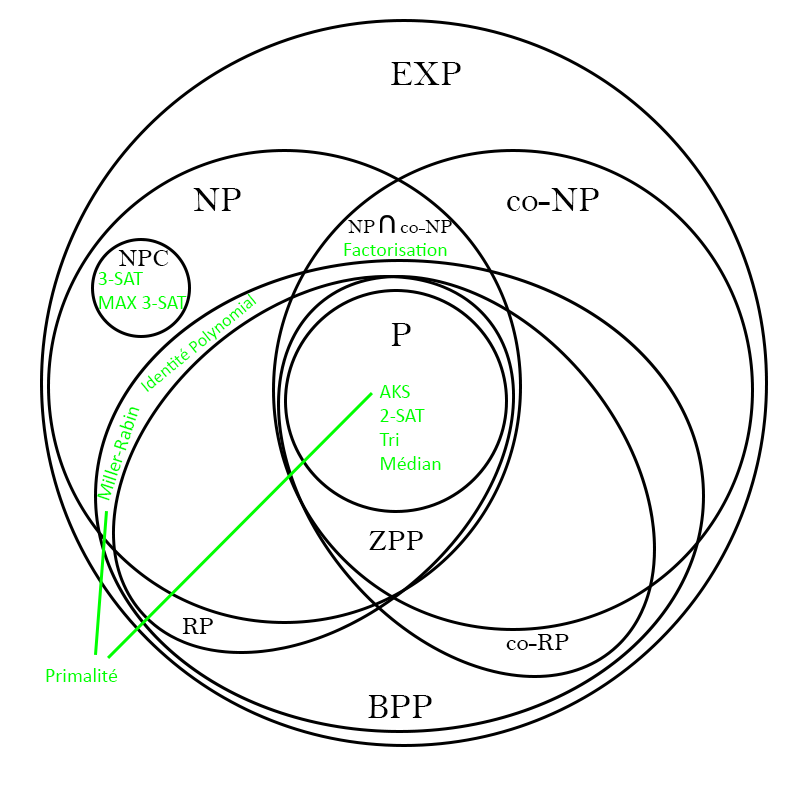
\includegraphics[width=0.65\textwidth]{classes.png}\\
	Relations entre les classes de complexité
\end{center}
\end{document}
% !TeX program = xelatex